\chapter{Pilotforsøg}\vspace{-.75cm}\label{pilot}
\section{Formål}
Pilotforsøget udføres med henblik på at kunne lave algoritmer ud fra målinger med et accelerometer og gyroskop, som adskiller de tre forskellige aktivitetsformer gang, løb og cykling. Det undersøges derudover hvilke af accelerometerets akser der er essentielle at lave algoritmer ud fra. Ydermere undersøges signalernes frekvens for at undgå aliasing i det endelige system og for at kende nyquistfrekvensen. Sidst undersøges hvilken indflydelse placering af sensoren har på signalets udformning. Dette gøres så det endelige systems signal ikke går i mætning på grund af for stor kraftpåvirkning, og for at undersøge om signalerne kan adskilles uanset hvilken af de tre placeringer der vælges.

Til opsamling af data, anvendes en Shimmer 3. Dette er en enhed, som indeholder flere sensorer, hvor der til forsøget benyttes et accelerometer og et gyroskop. 


%Resultaterne fra pilotforsøget bruges til at designe det endelige system, hvor softwaren for CY8CKIT-043 PSoC 4 M-Series Prototyping Kit skal konfigureres og tilpasses.

Formålet med pilotforsøget er dermed:\vspace{-3mm}
\begin{itemize}
\item At undersøge hvordan signalerne for gang, løb og cykling adskilles fra hinanden. 
\item At undersøge hvilken betydning placering af sensorene har for signalets udformning ved de tre aktivitetsformer gang, løb og cykling. 
\item At bestemme frekvensområdet for signalerne.
\item At bestemme amplitude for signalerne 
\end{itemize}
%er det nødvendigt at kende signalets frekvensindhold og vide, hvordan forskellige aktivitetsformer påvirker systemet. Målingerne skal undersøges for at kunne lave en algoritme, som kan få sensoren til at skelne imellem de pågældende aktivitetsformer. Derudover skal det bestemmes, hvor sensoren skal placeres på kroppen for mest optimalt udbytte. Derfor er formålet med pilotforsøget følgende:
%\begin{itemize}
%	\item Bestemme hvordan sensoren påvirkes af gang, løb og cykling. (Undersøge signalets udformning for accelerometer og gyroskop ved aktiviteterne; løb, gang og cykling. 
%		- Ligeledes at undersøge placeringen af sensoren ift. påvirkning af signalet.	
%	\item Undersøge hvor mange g-kræfter sensorens målinger ændrer sig alt efter placering på kroppen.
%	\item Undersøge bevægelsesmønstret i signalet i forhold til placering af sensor.
%	\item Bestemme frekvensindholdet for signalet.
%\end{itemize}

\section{Metode}
%Forsøgets metode er bestemt og udført med henblik på at opfylde pilotforsøgets formål. Dette involverer henholdsvis de materialer der skal benyttes samt den fremgangsmåde som ligger til grund for udførelsen.

Til forsøget medtages kun forsøgspersoner, som ikke lider af gener der forhindrer dem i at udføre aktiviteterne gang, løb og cykling. Er en person skadet eller syg, eksluderes denne dermed fra forsøget. Der udføres kun forsøg på gruppemedlemmer, og det er derfor ikke muligt at udføre forsøget på en person fra målgruppen, som er på 8-12 år. Resultaterne kan dermed variere i forhold til målgruppen, da disses vægt og højde vil varierer fra forsøgspersonerne. 

%Forsøget inkluderer udelukkende fuldt funktionsdygtige personer, hvormed ingen forsøgspersoner må have fysiske gener som kan medføre besvær ved udførsel af aktiviterne; gang, løb og cykling. Dermed sikres det, at forsøgets data indeholder normaliserede data som giver grundlag for et validt og repræsentativt datasæt for fysisk funktionsdygtige personer. 

Forsøget vil tage udgangspunkt i tre forudbestemte placeringer på underbenet af enheden, Shimmer3. Disse placeringer er udvalgt på baggrund af bevægelsesanalysen, hvor det ses at de største bevægelser optræder her i forbindelse med gang, løb og cykling. Accelerometet registrerer position og acceleration, og det forventes derfor at den største forskel vil kunne ses ved disse placeringer, da det især er denne del af benet, der bevæges under gang og løb. I databehandlingen behandles kun data fra accelerometerets x- og y-akse, da det kun er placering B der påvirkes af z-aksen ved aktiviteten gang, hvormed det formodes at samme påvirkning gælder for løb\citep{RueterboriesSpaichLarsenEtAl2010}. Ud fra bevægelsesanalysen i \secref{bevaegelse}, udledes det ligeledes at alle tre aktiviteter primært er i disse to retninger. 
% Dette vælges på baggrund af bevægelsesanalysen, hvor det blev udledt at den primære bevægelse af  benet ved de tre aktivitetsformer gang, løb og cykling i x- og y-aksens retning \citep{kilde}. \fxnote{måske noget om gyroskop + er det rigtigt i forhold til bevægelsesanalysen??}


% med henhold til æstetiske og brugervenlige aspekter samt \secref{TEORI SENSORER}. \newline
%\textit{Jeg ved ikke helt hvad jeg skal skrive vores begrundelse er ift. det teori om gyroskop, derfor skal de sidste linjer her skrives på senere. Ellers hvis en af jer ved nok om gyroskop til at skrive begrundelsen ;-)}
 

\subsection{Materialer}
\begin{itemize}
	\item Løbebånd med justerbar hastighed og sikkerhedsbæresele.
	\item Motionscykel.
	\item Shimmer3 sensor med tilhørende holder og strap.
	\item Sportstape.
	\item Computer med følgende software:
	\begin{itemize}
		\item Labview.
		\item Shimmer sensing.
	\end{itemize}
\end{itemize}

\section{Fremgangsmåde}
Forsøgets fremgangsmåde i to dele. Første del indeholder en opsætning af Shimmer3, mens den anden del er fremgangsmåden for optagelse af data fra forsøget.

\subsubsection{Opsætning af Shimmer3 SUB}
Før forsøgene kan udføres skal shimmer forbindes korrekt med computeren, og indstilles til at bruge de sensorer der ønskes i pilotforsøget. \vspace{-3mm}
\begin{itemize}
	\item Shimmer forbindes til programmet Labview gennem bluetooth.
	\item Shimmer indeholder en række sensorer, hvorad føægende skal aktiveres: 
		\begin{itemize}
			\item Widerange Accelerometer.
			\item Gyroscope.
		\end{itemize}
	\item De maksimale arbejdsområder på $\pm$16 G og $\pm$2000 dps vælges, da signalets amplitude endnu er ukendt.
	\item Samplingsfrekvensen indstilles på 512 Hz, da signalets frekvens er ukendt, og denne samplingsfrekvens er den maksimale der kan vælges, når både gyroskopet og accelerometeret er i brug.  
	\item Det er nu muligt at starte stream, og derefter realtime.
	
	 
\end{itemize}



%Shimmer3 undersøges nu for at kunne konkludere hvorvidt værdierne fra sensorerne er korrekte. Til denne undersøgelse skal akserne for accelerometeret og gyoskopet findes ved opslag i datablad for enheden. Når disse akser er bestemt, benyttes Labview til at optage målinger i. Der startes en ’Stream’ for at undersøge realtime målingerne.
%Først undersøges accelerometerets værdier ved at placere Shimmer3 på en flad, fast overflade. Shimmer3 vendes i 6 forskellige positioner afhængigt af om det er den positive eller negative akse for x, y eller z som undersøges. Værdien for den positive akse for henholdsvis x, y og z skal vise cirka 9,8 m/s, og med negativt fortegn ved den negative akse for x, y og x. I tilfælde af at værdierne er cirka 9,8 m/s, da kan accelerometerets nøjagtighed godtages. Ydermere undersøges gyroskopet ved at spinne Shimmer3 rundt i en række forskellige retninger for at undersøge hvorvidt sensoren reagerer på dette. Hvis gyroskopet registrerer ændringerne, da godtages dennes nøjagtighed. 
%Shimmer3 er forbundet, konfigureret og undersøgt således forsøget efterfølgende kan gennemføres.

\subsection{Udførsel af forsøget}
Forsøget udføres på fire forsøgspersoner, som alle skal udføre aktiviteterne gang, løb og cykling. Den nedenstående beskrivelse af forsøgets fremgangsmåde er gældende for én af de forudbestemte placeringer af Shimmer3 på forsøgspersonens højre ben. Dog benyttes den samme fremgangsmåde til de resterende to placeringer. De tre placeringer kan ses på \figref{fig:sensor_placering}

\begin{figure}[H]
	\centering
	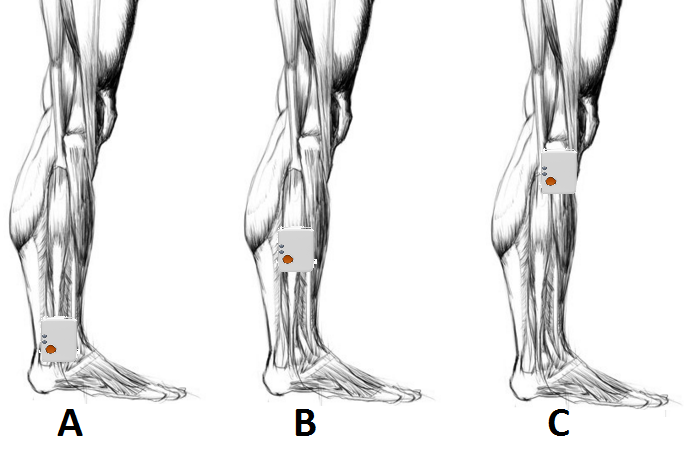
\includegraphics[scale=0.6]{figures/qBilag/Sensor_placering2.png}
	\caption{På figuren ses, hvor sensoren skal placeres under pilotforsøget. Placering A: proximalt for den laterale malleolus. Placering B: medialt på den laterale side af tibia. Placering C: distalt for patella på den laterale side. (Modificeret fra \cite{Perna2016,Shimmer2016})}
	\label{fig:sensor_placering}
\end{figure}

Inden forsøget skal forsøgspersonen fastspændes i en sikkerhedssele, så der ikke opstår skader hvis personen snubler på løbebåndet. Derudover skal forsøgspersonen inden hver måling fortælle hvor på borgskalaen denne befinder sig og er det under 11\fxnote{var det 11?} kan målingen påbegyndes. Denne værdi er valgt for at forsøgspersonen ikke allerede har det som om kroppen er i gang med træning, og det dermed sikres at alle forsøgspersoner har samme startbetingelser for alle forsøg. Borgskalaen der benyttes til pilotforsøget kan ses på \figref{fig:borgskala}. 

\begin{figure}[H]
	\centering
	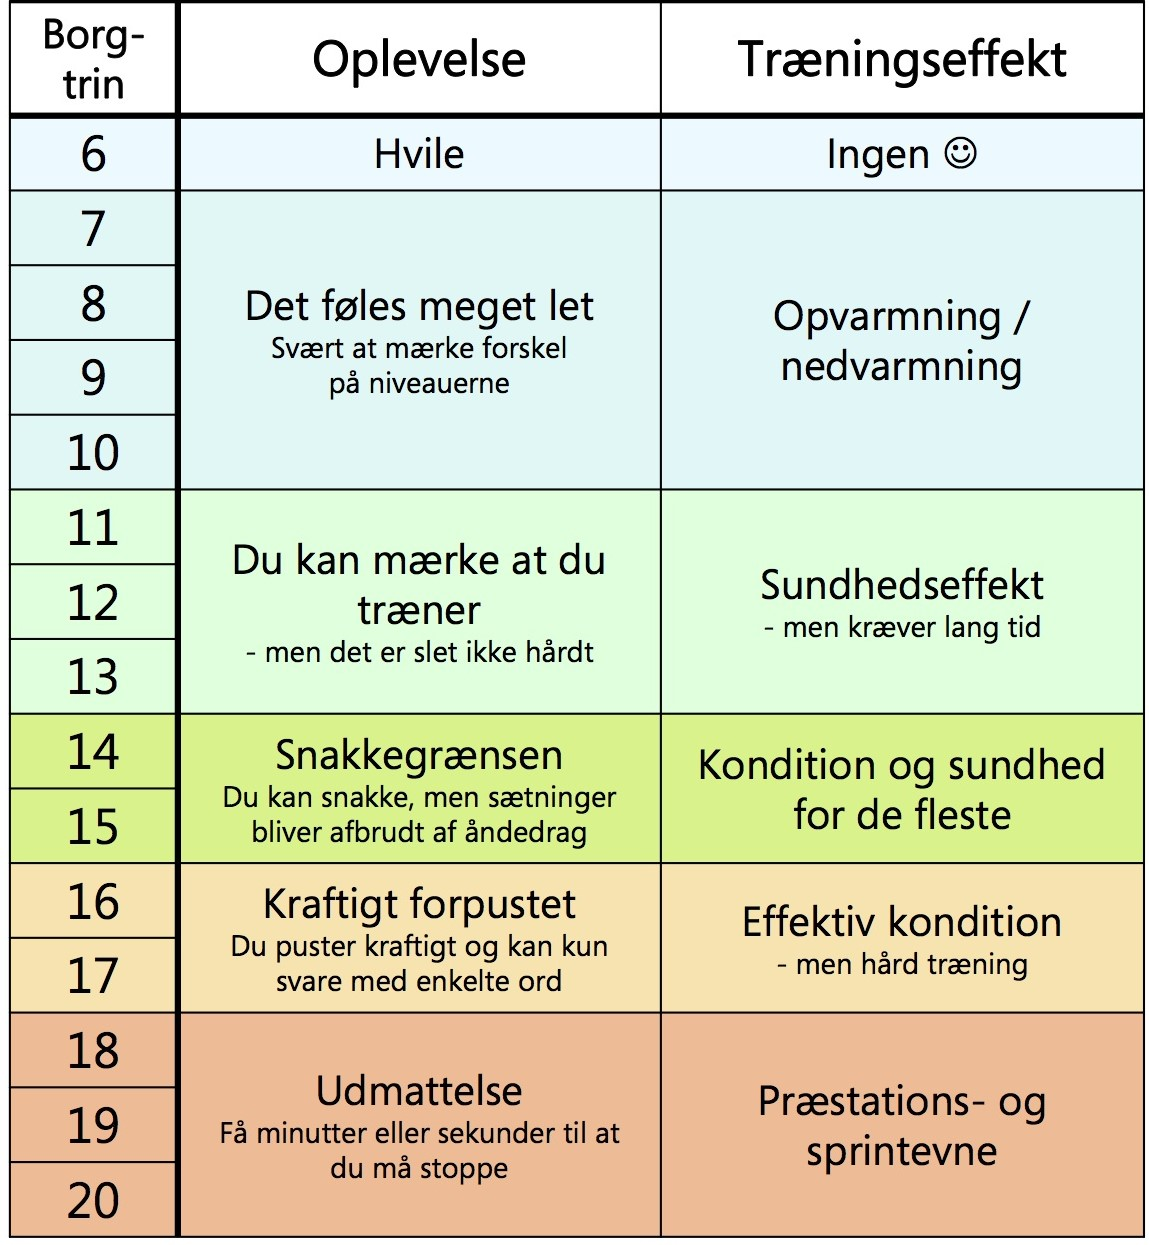
\includegraphics[scale=0.5]{figures/qBilag/Borg-skala.jpg}
	\caption{På figuren ses borgskalaen, som er den der benyttes inden forsøgsstarten. (Modificeret)\cite{Patientinformationen2013})}
	\label{fig:borgskala}
\end{figure}

Første måling er gang, hvor et middel gangtempo på 4,8 km/t er valgt\citep{Miles2007}. \vspace{-3mm}
\begin{itemize}
		\item Der foretages en baseline på 10 sekunder, hvor forsøgspersonen skal stå oprejst med ret ryg og fødderne placeret parallelt og kigge ligefrem ved baseline målingen.
		\item Løbebåndet indstilles til 4,8 km/t, hvor forsøgspersonen går på løbebåndet indtil en konstant hastighed på løbebåndet opnås. 
%		\item Forsøgspersonen indikerer når denne føler en homogen bevægelses-cyklus.
		\item Målingen på 45 sekunder igangsættes.
		\item Fremgangsmåden gentages for alle tre placeringer. 
\end{itemize}
 
Anden måling er løb, et middel løbetempo på 11,3 km/t er valgt\citep{Miles2007}. \vspace{-3mm}
\begin{itemize}
	\item Der foretages en baseline på 10 sekunder, hvor forsøgspersonen skal stå oprejst med ret ryg og fødderne placeret parallelt og kigge ligefrem ved baseline målingen.
	\item Løbebåndet indstilles til 11,3 km/t, hvor forsøgspersonen løber på løbebåndet indtil en konstant hastighed på løbebåndet opnås. 
%	\item Forsøgspersonen indikerer når denne føler en homogen bevægelses-cyklus.
	\item Målingen på 45 sekunder igangsættes.
	\item Fremgangsmåden gentages for alle tre placeringer.
\end{itemize}
 
Tredje måling er cykling, hvor et cykeltempo på 20,9 km/t er valgt, hvilket er et højt cykeltempo\citep{Miles2007}. Tempoet er dog underordnet, da der kun ønskes at se på forskellen i selve bevægelsen fra de andre aktivitetsformer. \vspace{-3mm}
\begin{itemize}
	\item Der foretages en baseline på 10 sekunder, hvor forsøgspersonen skal sidde i en naturlig cykelposition på motionscyklen med begge fødder på pedalerne, hvoraf den højre pedal skal være helt i bund. Denne position er valgt, da den er mulig at lave tilnærmelsesvis ens for alle forsøgspersoner, hvormed de får den samme baseline.
	\item Forsøgspersonen træder i pedalerne indtil denne opnår en konstant hastighed på 20,9 km/t ved en belastning på 35 W. Dermed sikres det at alle forsøgspersoner bruger den samme belastning gennem forsøget.  
	\item Målingen på 45 sekunder igangsættes. 
	\item Fremgangsmåden gentages for alle tre placeringer.
\end{itemize}

Sidste måling foretages på løbebåndet, hvor forsøgspersonen gradvist skal stige i tempo under hele forsøget. Der noteres under forsøget hvornår forsøgspersonen skifter fra gang til løb.  \vspace{-3mm}
\begin{itemize}
	\item Der foretages en baseline på 10 sekunder, hvor forsøgspersonen skal stå oprejst med ret ryg og fødderne placeret parallelt og kigge ligefrem ved baseline målingen.
	\item Målingen igangsættes.
	\item Løbebåndet indstilles til 2 km/t, hvor forsøgspersonen skal gå i 20 sekunder.  
	\item Hastigheden stiger herefter med 2 km/t for hvert 20. sekund, indtil forsøgspersonen har opnået maksimal hastighed, eller løbebåndets maksimale hastighed. 
	\item Målingen stoppes. 
	\item Fremgangsmåden gentages for alle tre placeringer.
\end{itemize}


\section{Databehandling}
\textit{indledning}


\subsection{Kalibrering af shimmer}
Forud for pilotforsøgets målinger blev Shimmer kalibreret og testet. For at undersøge hvorvidt kalibreringen af Shimmer fungerede optimalt, blev der opsamlet data til at be-, eller afkræfte dette. Data fra de tre akser, x, y og z blev behandlet. \\
Når Shimmer er placeret i en kalibreringsboks på et bord med henblik på en respektiv akse, bør accelerometeret blive påvirket med $\pm 1$G, mens de resterende akser ikke bør påvirkes.

\begin{figure}[H]
	\centering
	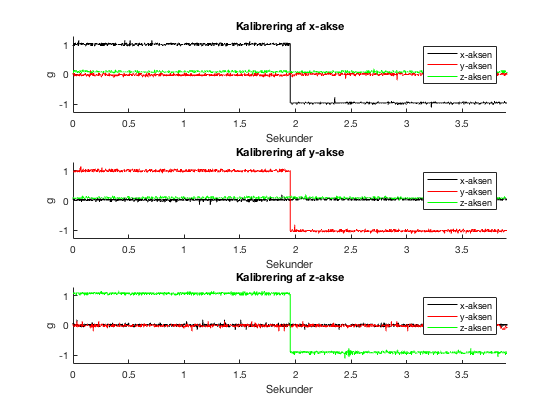
\includegraphics[scale=0.68]{figures/qBilag/kalibreringsdata}
	\caption{På figuren ses kalibreringsdataene tilhørende accelerometerets x, y og z-akse.}
	\label{fig:Ap_Kalibrering}
\end{figure}

For hver akse blev den gennemsnitlige værdi for henholdsvis den positive- og negative akse beregnet. Dette resulterede i at x-aksen gennemsnitlig afveg henholdsvis 3,5\% i den negative akse og -2,2\% i den positive akse. Y-aksen afveg gennemsnitligt -2,6\% i den negative akse og -0,6\% i den positive akse. Z-aksen afveg  gennemsnitligt med 8,8\% i den negative akse og 8,0\% i den positive akse.

\subsection{Baseline af gang, løb og cykling}
Forud for hver enkelt måling blev der foretaget en baselinemåling som indikation for hvorvidt Shimmer fungerede forud for aktiviteten. Dataene skal afspejle en tilnærmelsesvis fuldstændig tyngdekraftpåvirkning på accelerometerets y-akse, som resultat af Shimmers placering på benet.

\begin{table}[H]
	\centering
	\begin{tabular}{cccc}
		\hline
		\rowcolor[HTML]{C0C0C0} 
		{\color[HTML]{333333} Forsøgsperson} & {\color[HTML]{333333} \begin{tabular}[c]{@{}c@{}}Placering A, \\ y-akse {[}G{]}\end{tabular}} & {\color[HTML]{333333} \begin{tabular}[c]{@{}c@{}}Placering B,\\ y-akse {[}G{]}\end{tabular}} & {\color[HTML]{333333} \begin{tabular}[c]{@{}c@{}}Placering C,\\ y-akse {[}G{]}\end{tabular}} \\ \hline
		F1 & 0,98 & 0,99 & 0,97 \\ \hline
		F2 & 1 & 0,99 & 0,96 \\ \hline
		F3 & 0,98 & 0,98 & 0,98 \\ \hline
		F4 & 0,97 & 0,99 & 0,95 \\ \hline
	\end{tabular}
	\caption{I tabellen ses de gennemsnitlige baselineresultater fra accelerometerets y-akse forud for gang.}
	\label{fig:Ap_baselinegang}
\end{table}\vspace{-0.5cm}

\begin{table}[H]
	\centering
	\begin{tabular}{cccc}
		\hline
		\rowcolor[HTML]{C0C0C0} 
		{\color[HTML]{333333} Forsøgsperson} & {\color[HTML]{333333} \begin{tabular}[c]{@{}c@{}}Placering A, \\ y-akse {[}G{]}\end{tabular}} & {\color[HTML]{333333} \begin{tabular}[c]{@{}c@{}}Placering B,\\ y-akse {[}G{]}\end{tabular}} & {\color[HTML]{333333} \begin{tabular}[c]{@{}c@{}}Placering C,\\ y-akse {[}G{]}\end{tabular}} \\ \hline
		F1 & 0,99 & 0,99 & 0,97 \\ \hline
		F2 & 0,99 & 0,99 & 0,96 \\ \hline
		F3 & 0,97 & 0,98 & 0,98 \\ \hline
		F4 & 0,97 & 0,99 & 0,95 \\ \hline
	\end{tabular}
	\caption{I tabellen ses de gennemsnitlige baselineresultater fra accelerometerets y-akse forud for løb.}
	\label{fig:Ap_baselineloeb}
\end{table}\vspace{-0.5cm}

Ved cykling benyttes gyroskopets data, da cykling detekteres som en roterende bevægelse omkring z-aksen. Enheden af dataet heraf er grader per sekund (dps), og dermed bør baselineresultaterne ligge omkring nul.
\begin{table}[H]
	\centering
	\begin{tabular}{cccc}
		\hline
		\rowcolor[HTML]{C0C0C0} 
		{\color[HTML]{333333} Forsøgsperson} & {\color[HTML]{333333} \begin{tabular}[c]{@{}c@{}}Placering A, \\ z-akse {[}dps{]}\end{tabular}} & {\color[HTML]{333333} \begin{tabular}[c]{@{}c@{}}Placering B,\\ z-akse {[}dps{]}\end{tabular}} & {\color[HTML]{333333} \begin{tabular}[c]{@{}c@{}}Placering C,\\ z-akse {[}dps{]}\end{tabular}} \\ \hline
		F1 & -0,98 & -0,83 & -0,87 \\ \hline
		F2 & -0,90 & -0,79 & -0,77 \\ \hline
		F3 & -0,68 & -0,58 & -0,99 \\ \hline
		F4 & -0,89 & -0,92 & -0,85 \\ \hline
	\end{tabular}
	\caption{I tabellen ses de gennemsnitlige baselineresultater fra gyroskopets z-akse forud for cykling.}
	\label{fig:Ap_baselinecykling}
\end{table}\vspace{-0.5cm}

\subsection{Maksimal g-påvirkning under gang, løb og hastighed}
Dataene fra aktiviteterne, gang, løb og hastighed blev alle behandlet med henblik på bestemmelse af den maksimale G påvirkning heraf. Dette blev bestemt af den maksimale peak-to-peak, for alle aktiviteter samt placeringer. Dataene blev kun behandlet med henblik på accelerometerets y-akse, som resultat af \secref{bevaegelse}. Enheden for et accelerometer forekommer i $\frac{m}{s^{2}}$, og dermed skal dette divideres med tyngdekraften for at omregne til G. 

\begin{table}[H]
	\centering
		\begin{tabular}{ccccc}
			\hline
			\rowcolor[HTML]{C0C0C0} 
			Forsøgsperson & Baseline neutral & \begin{tabular}[c]{@{}c@{}}Peak-to-Peak:\\ Placering A {[}G{]}\end{tabular} & \begin{tabular}[c]{@{}c@{}}Peak-to-Peak:\\ Placering A {[}G{]}\end{tabular} & \begin{tabular}[c]{@{}c@{}}Peak-to-Peak:\\ Placering A {[}G{]}\end{tabular} \\ \hline
			F1 & (x), (x), (x) & 2,41 & 2,32 & 3,68 \\ \hline
			F2 & (x), (x), (x) & 3,38 & 3,48 & 3,81 \\ \hline
			F3 & (x), (x), (x) & 3,77 & 3,77 & 2,70 \\ \hline
			F4 & (x), (x), (x) & 2,90 & 3,91 & 4,01 \\ \hline
		\end{tabular}%
	\caption{I tabellen ses de maksimale peak-to-peak resultater fra accelerometerets y-akse som resultat af gang. Den maksimale peak-to-peak er fundet for både placering a,b og c. Baseline neutral (x) indikerer at baselinemålingen var som forventet forud for målingen.}
	\label{fig:Ap_maxggang}
\end{table}

\begin{table}[H]
	\centering
	\begin{tabular}{ccccc}
		\hline
		\rowcolor[HTML]{C0C0C0} 
		Forsøgsperson & Baseline neutral & \begin{tabular}[c]{@{}c@{}}Peak-to-Peak:\\ Placering A {[}G{]}\end{tabular} & \begin{tabular}[c]{@{}c@{}}Peak-to-Peak:\\ Placering A {[}G{]}\end{tabular} & \begin{tabular}[c]{@{}c@{}}Peak-to-Peak:\\ Placering A {[}G{]}\end{tabular} \\ \hline
		F1 & (x), (x), (x) & 10,6 & 7,87 & 7,43 \\ \hline
		F2 & (x), (x), (x) & 6,32 & 8,64 & 11,0 \\ \hline
		F3 & (x), (x), (x) & 7,68 & 7,43 & 8,06 \\ \hline
		F4 & (x), (x), (x) & 9,90 & 11,4 & 11,8 \\ \hline
	\end{tabular}%
	\caption{I tabellen ses de maksimale peak-to-peak resultater fra accelerometerets y-akse som resultat af løb. Den maksimale peak-to-peak er fundet for både placering a,b og c. Baseline neutral (x) indikerer at baselinemålingen var som forventet forud for målingen.}
	\label{fig:Ap_maxgloeb}
\end{table}

\begin{table}[H]
	\centering
	\begin{tabular}{ccccc}
		\hline
		\rowcolor[HTML]{C0C0C0} 
		Forsøgsperson & Baseline neutral & \begin{tabular}[c]{@{}c@{}}Peak-to-Peak:\\ Placering A {[}G{]}\end{tabular} & \begin{tabular}[c]{@{}c@{}}Peak-to-Peak:\\ Placering A {[}G{]}\end{tabular} & \begin{tabular}[c]{@{}c@{}}Peak-to-Peak:\\ Placering A {[}G{]}\end{tabular} \\ \hline
		F1 & (x), (x), (x) & 11,2 & 10,9 & 13,6 \\ \hline
		F2 & (x), (x), (x) & 14,1 & 15,0 & 17,2 \\ \hline
		F3 & (x), (x), (x) & 15,4 & 17,7 & 14,3 \\ \hline
		F4 & (x), (x), (x) & 25,8 & 23,8 & 23,4 \\ \hline
	\end{tabular}%
	\caption{I tabellen ses de maksimale peak-to-peak resultater fra accelerometerets y-akse som resultat af hastighed. Den maksimale peak-to-peak er fundet for både placering a,b og c. Baseline neutral (x) indikerer at baselinemålingen var som forventet forud for målingen.}
	\label{fig:Ap_maxghastighed}
\end{table}

I \secref{app:maxg} bestemmes det at resterende databehandling udelukkende omhandler placering A.


\subsection{Frekvensindhold}
Dataene fra aktiviteterne, gang og løb blev behandlet for at bestemme signalernes frekvensindhold, med henblik på bestemmelsen af samplingsfrekvensen. Der blev foretaget en frekvensdomæne analyse, hvilket muliggør visualisering af signalets magnitude ved forskellige frekvenser. 

\begin{figure}[H]
	\centering
	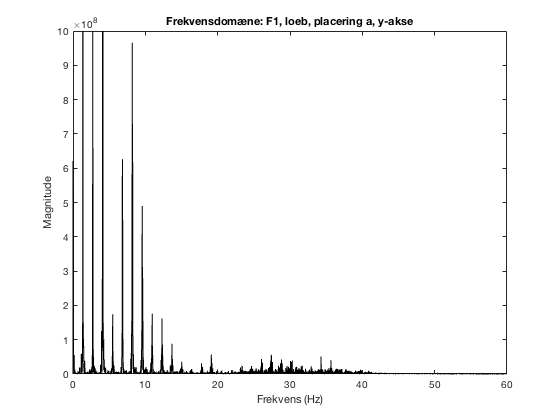
\includegraphics[scale=0.68]{figures/bProblemloesning/fft_f1_loeb}
	\caption{På figuren ses frekvensdomænet af aktiviteten løb for forsøgsperson 1.}
	\label{fig:Ap_FFt}
\end{figure}
Frekvensdomæneanalysen vises kun for denne forsøgsperson da frekvensspektrummet var størst heraf. Dette gøres da systemets samplingsfrekvens bestemmes med i forhold til på den højeste frekvens.

\subsection{Filtrering af gang, løb og hastighed}
\textbf{ikke lavet endnu}

\section{Resultater}
\textit{Indledning}
\subsection{Kalibrering af shimmer}
Resultatet af databehandlingen bevirker at kalibreringen af Shimmer antages at være tilstrækkelig. Dette antages at være tilstrækkeligt, da y-aksen  afviger med 1,6\% fra den teoretiske værdi. En eventuel fejlkilde til at denne fejlmargin forekom, kunne være at bordet hvorpå Shimmer var placeret, ikke var i vatter.

\subsection{Baseline af gang, løb og cykling}
Baselinemålingerne for henholdsvis gang og løb resulterede i en enslignende påvirkning. Som forventet var G påvirkningen ikke 1G, hvilket er et resultat af at Shimmer ikke er placeret ortogonalt på y-aksen, på benet. Resultaterne fra disse målinger indikerer altså Shimmer har optaget data som stemmer overens med antagelsen om den tilnærmelsesvise påvirkning på 1G. 

Resultaterne fra baselinemålingerne vedrørende cykling ligger som forventet omkring nul, hvilket er et resultat af at Shimmer ikke er blevet påvirket i z-aksen i nogen væsentlig grad, da benet ikke bevæges. Resultaterne af disse målinger indikerer at Shimmer har optaget data som stemmer overens med antagelsen om den tilnærmelsesvise påvirkning på 0 dps. 

\subsection{Maksimal g-påvirkning under gang, løb og hastighed} \label{app:maxg}
Resultatet af databehandlingen vedrørende de tre aktiviteter med henblik på bestemmelsen af den maksimale G påvirkning, medførte at hastigheds aktiviteten havde den største påvirkning. Resultaterne fra placering A, B eller C overskrider ikke $\pm 16G$, hvoraf den mest fordelagtige placering frit kan vælges. Med baggrund i \secref{succeskrav} og \secref{funktionellekrav} skal placeringen ikke være til gene for barnet, den skal altså nemt af-, og påmonteres, hvoraf placering A er valgt. Dette medfører at den videre resultatbehandling tager udgangspunkt i placering A. 

\subsection{Frekvensindhold}
Databehandlingen af frekvensindholdet fra gang og løb medførte at det største frekvensspektrum lå mellem 0 og 45Hz. Dette medfører at det endelige systems samplingsfrekvens kan bestemmes. I følge Nyquist skal samplingsfrekvensen være dobbelt så stor som signalets maksimale frekvens. Dette er en teoretisk værdi, og i praksis bør samplingsfrekvensen være 20 gange større. \\
Det endelige system skal altså have en samplingsfrekvens på 900Hz.

\subsection{Filtrering af gang, løb og hastighed}
ikke lavet. 
\section{Diskussion}

\section{Konklusion}

%% Opgaver - rettelser
% Man skal markere på forsøgspersonen med tush eller andet hvor sensoren skal placeres